\chapter{Belle II experiment}
\section{Belle II and SuperKEKB overview}
The goal of the Belle II experiment is to search for evidence of New Physics, and the expected operation period is from 2019 to the end of 2030. The facilities are located in KEK, Tsukuba City, around 70 km in the north of Tokyo, Japan. The SuperKEKB accelerator enables electron-positron collision at the center-of-mass energy on the region of $\Upsilon(4S)$ resonance which is just above the mass of two $B$ mesons. The electron and positron beams are designed at 7 GeV and 4 GeV, respectively, with a boost factor of 0.28, providing an environment for measuring time-dependent $CP$ violation by displacing the decay vertices of a $B$ meson pair in a measurable distance along the boosted direction. The SuperKEKB has a targeted luminosity of $8\times 10^{35}\: \text{cm}^{-2} \text{s}^{-1}$, a factor of 40 times higher than its predecessor, the KEKB.  Some key parameters of the SuperKEKB are listed in Table \ref{tab:superkekb_pars}. The schematic view of SuperKEKB and Belle II are shown in Figure \ref{fig:superkekb_belle2}.

\begin{figure}
	\centering 
	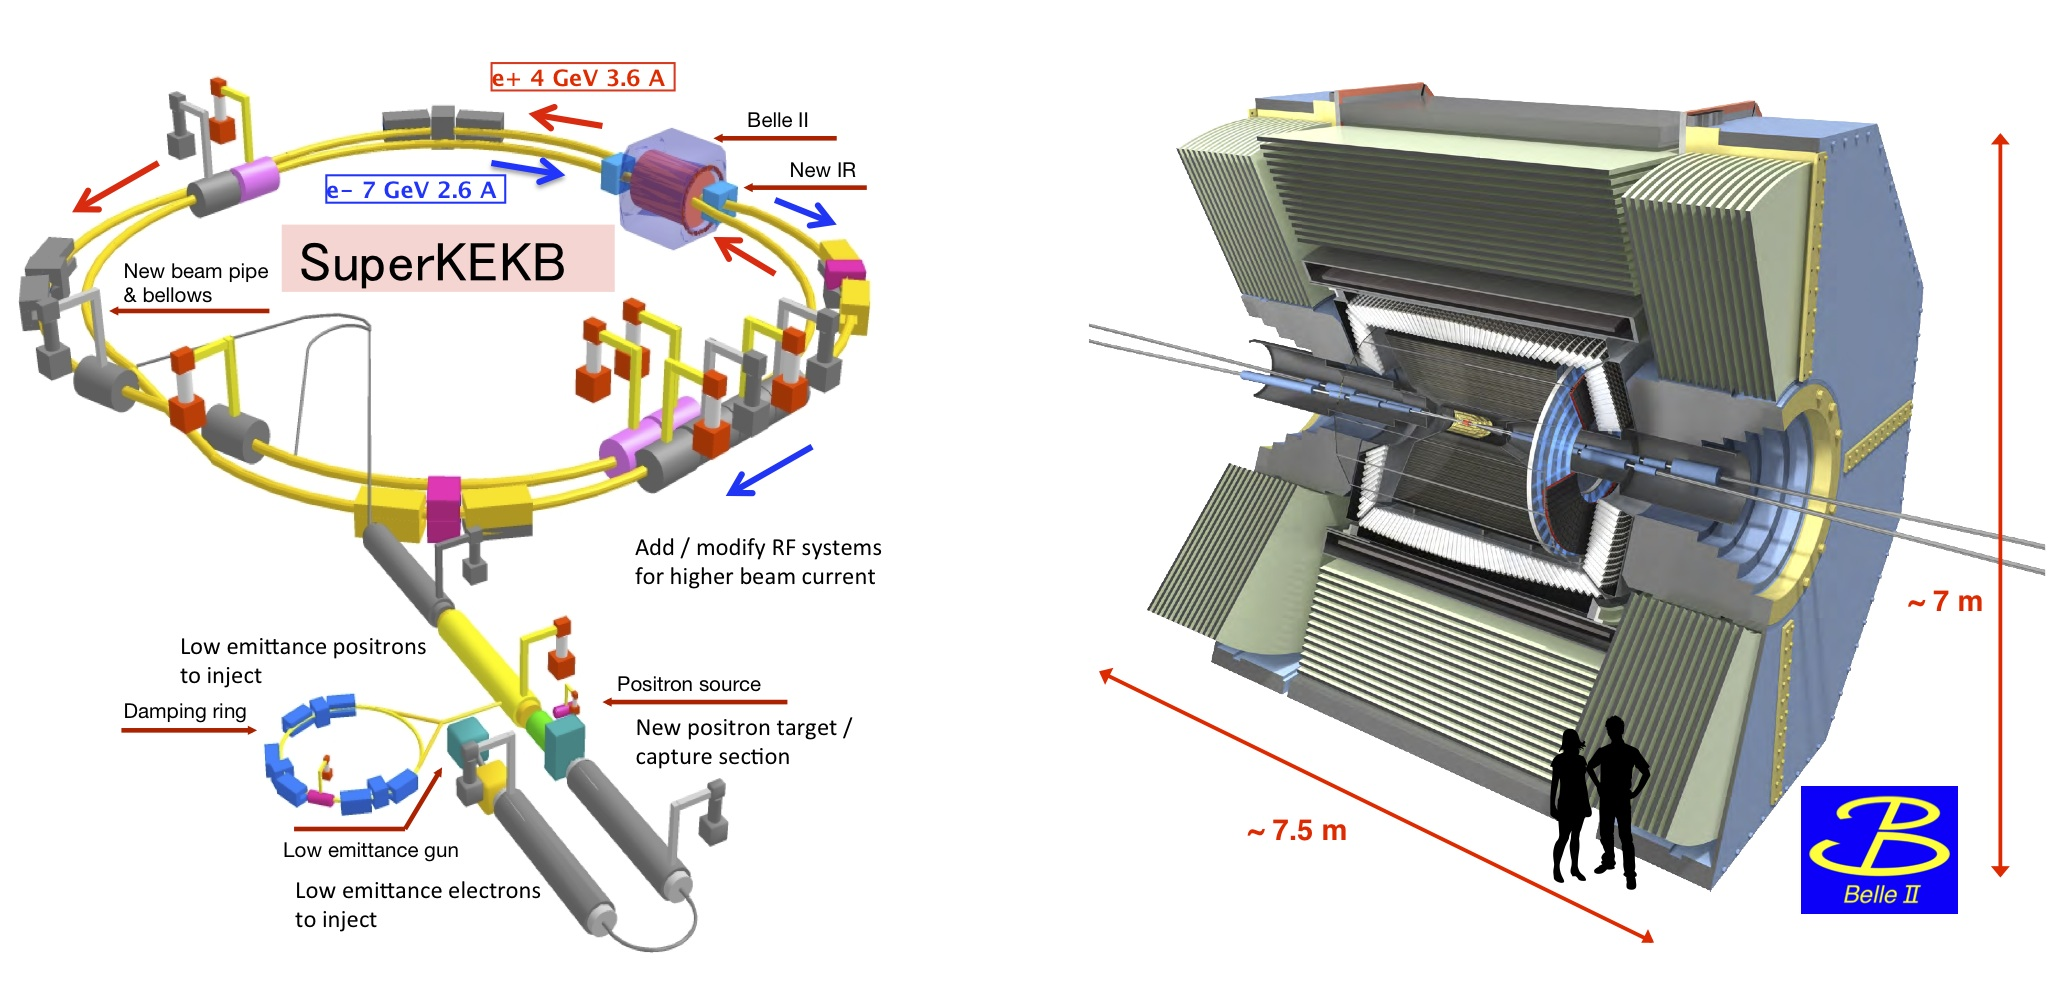
\includegraphics[height=7cm]{SuperKEKB-BelleII.jpg}
	\caption{The schematic view of SuperKEKB and Belle II detector~\cite{Abe:2010gxa}.}
	\label{fig:superkekb_belle2}
\end{figure}

\begin{table}[H]
	\centering
	\large
	\caption{SuperKEKB parameters for low energy (LER) and high energy (HER) rings~\cite{b2book}.}
	\label{tab:superkekb_pars}
	\begin{tabular}{c c c c}
		\toprule
		
		Parameters & LER ($e^+$) & HER ($e^-$) & Unit\\
		\hline
		Energy & 4.0 & 7.0 & GeV\\
		Half crossing angle & \multicolumn{2}{c}{41.5} & mrad\\
		Horizontal emittance & 3.2 & 4.6 & nm \\
		Emittance ratio & 0.27 & 0.25 & \%\\
		Beta functions at IP ($x$/$y$) & 32/0.27 & 25/0.30 & mm\\
		Beam currents & 3.6 & 2.6 &  A \\
		Beam–beam parameter & 0.0881 & 0.0807 & {}\\
		Luminosity & \multicolumn{2}{c}{$8\times 10^{35}$} &  $\text{cm}^{-2} \text{s}^{-1}$\\
		Perimeter of ring & \multicolumn{2}{c}{3} & km\\
		
		\bottomrule
	\end{tabular}
\end{table}


The Belle II detector has a close size as the Belle detector so that it is placed in the same shell, but all sub-detectors and electronic systems have been either newly built or considerably upgraded. The advantage of the SuperKEKB requires that the Belle II has to be able to stably operate at a 40 times higher event rates as well as 10 to 20 times higher beam background compared to that in the Belle. The mitigation of the effects caused by such high beam background is essential to the success of the Belle II. Higher background level leads to higher occupancy and radiation damage to the detectors, along with more fake hits in the vertex detectors and central drift chamber, pile-up backgrounds in electromagnetic calorimeter and neutron-induced hits in muon detector. Data-acquisition system (DAQ) and trigger are also upgraded not only to adapt to higher luminosity but also for a better low-multiplicity event sensitivity. The Belle II detector in the top view is shown in Figure \ref{fig:belle2_view}.

\begin{comment}
 and expected performances are summarized as follows: 


\textbullet \space vertex resolution of $B$ mesons of $\sim 50 \: \mu\text{m}$,

\textbullet \space excellent reconstruction efficiency for charged tracks down to several 100 MeV and fairly good efficiency for charged tracks down to $\sim$ 50 MeV,

\textbullet \space excellent momentum resolution up to 8 GeV/c,

\textbullet \space highly efficient particle identification to separate $\pi^{\pm}$, $\mu^{\pm}$, $e^{\pm}$, $K^{\pm}$ and $p$ at full energy range of experiment,

\textbullet \space full cover of experimental acceptance solid angle,

\textbullet \space ultra fast and highly efficiency DAQ and trigger system to cope with large data quantities and fast triggering frequency. 
\end{comment}

\begin{figure}[htbp]
	\centering 
	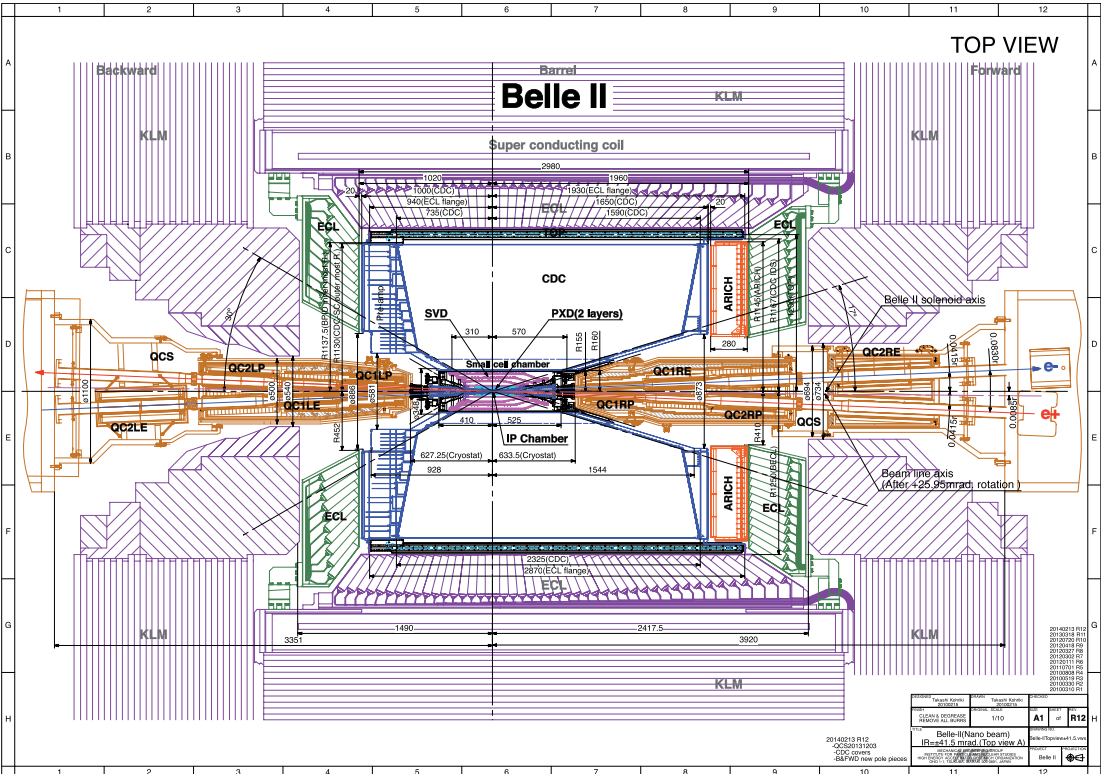
\includegraphics[height=10cm]{Belle2TopView.png}
	\caption{The Belle II detector top view~\cite{b2book}.}
	\label{fig:belle2_view}
\end{figure}

The success of the Belle II detector depends on the complex of sub-detectors where each of them is design for specific purposes. The critical components and features are explained in the following sections. 

\section{Vertex detector (VXD)}
The vertex detector is composed of two detectors, the silicon based pixel detector (PXD) and silicon based vertex detector (SVD), where total 6 layers are placed in the inner-most region from interaction point (IP).  The geometry of VXD is shown in Figure \ref{fig:svdgeo}. The PXD is placed at a radii of $r=14$ mm and $r=22$ mm with DEPFET~\cite{Abe:2010gxa} type pixel sensors, which is designed to provide two dimensional hit position information. The inner layer leaves a sufficient space for possible variations of the beampipe layout. The size of two layers are determined by the required acceptance angle from 17 degrees (forward) to 150 degrees (backward). The pixel sensor is a monolithic structure with current-digitizing electronics at the end of the senor that makes a very thin  layer at about 50 microns. The schematic view of sensors on PXD is shown in Figure \ref{fig:pxd}.
\begin{figure}[htpb]
	\centering
	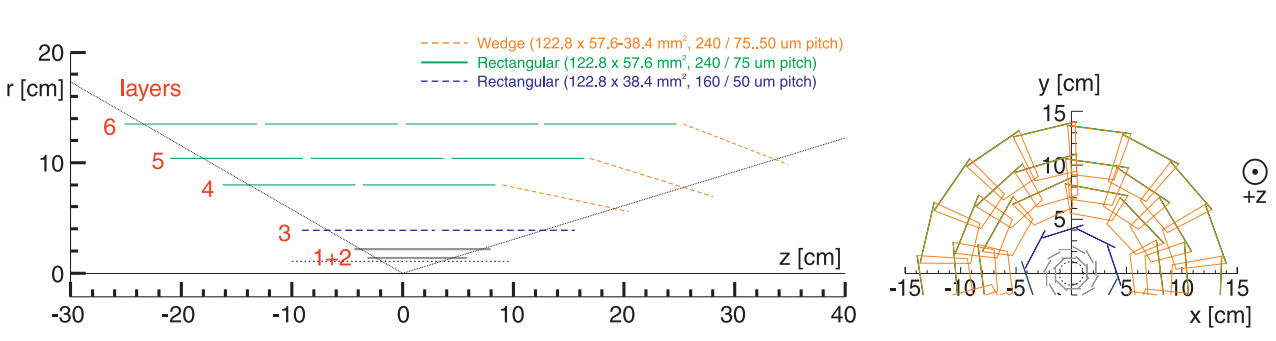
\includegraphics[height=5cm, width=1\linewidth]{VXDGEO.png}
	\caption{A schematic view of of PXD and SVD. Two PXD layers are in grey, SVD layer 3 is in blue and layer 4, 5, 6 are in green~\cite{Abe:2010gxa}.}
	\label{fig:svdgeo}
\end{figure}
\begin{figure}[htpb]
\centering
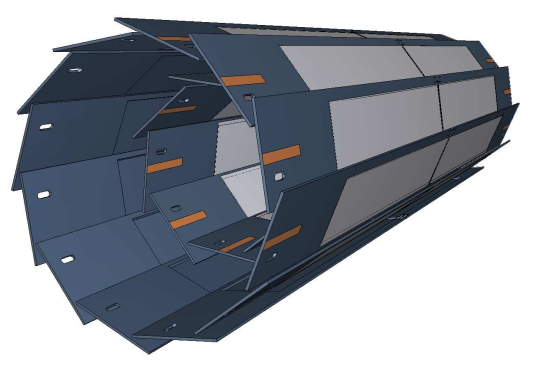
\includegraphics[width=0.6\linewidth]{pxd}
\caption{The geometry of sensors on PXD where the light grey surfaces are DEPFET sensors with a thinness of 50 microns. The full length including the out modules is 174 mm~\cite{Abe:2010gxa}. }
\label{fig:pxd}
\end{figure}
 As the very close range the PXD is, the sensors are exposed to a very high event rate and very high beam background environment. The large data flow from PXD without any data reduction scheme is problematic for data acquisition system. In order to reduce the data that is not interested by physics analysis such as beam backgrounds, a fast online tracking system is built up for searching a ``region of interest" (ROI) on the PXD sensors. To be specific, the data from PXD will be first readout to a system called ``ONSEN" which can store large size temporary data up to 5 seconds. In this timing window, a fast online tracking system will perform a track fitting using vertext detector and central drift chamber to extrapolate the fitted tracks backward to PXD plane so the ROI on the PXD sensors can be defined. The data from PXD outside of the ROI is not read out to external tapes where offline data is written. 

SVD detector consists of 4 layers of detectors called  ``double-sided silicon strip detectors" (DSSDs) at 39 mm, 80 mm, 104 mm, and 135 mm away from IP, respectively. The two sides of the sensors are called $p$-side and $n$-side, where the former is for the strips on $r-\phi$ direction (transverse direction) and the latter is for the strips on the $z$ direction (beamline direction). To suppress the background hits, a readout chip with a fast shaping time of $\mathcal{O}$(50 ns) is indispensable. The APV25 chip~\cite{french2001design} is chosen as the readout chip that was originally developed for CMS silicon tracker, with total 128 identical channels of low-noise preamplifiers followed by a 50 ns peaking time shaper stage. The polar angular acceptance ranges from 17 degrees to 150 degrees, which is asymmetric to account for the
forward boost of the center-of-mass frame. The combination between sensors, electronics and the supporting structure uses so-called ``Origami" concept that stands for a chip-on-sensor design, as shown in Figure \ref{fig:origami}. In the Origami scheme, the readout chips APV25 are placed on a single flexible circuit mounted on the $n$-side of the sensors. The channels of $p$-side are attached by small flexible fan-outs wrapped around the edge of the sensors. All connections between flex pieces, sensor, and APV25 chips are made by wire bonds.
\begin{figure}[htpb]
	\centering
	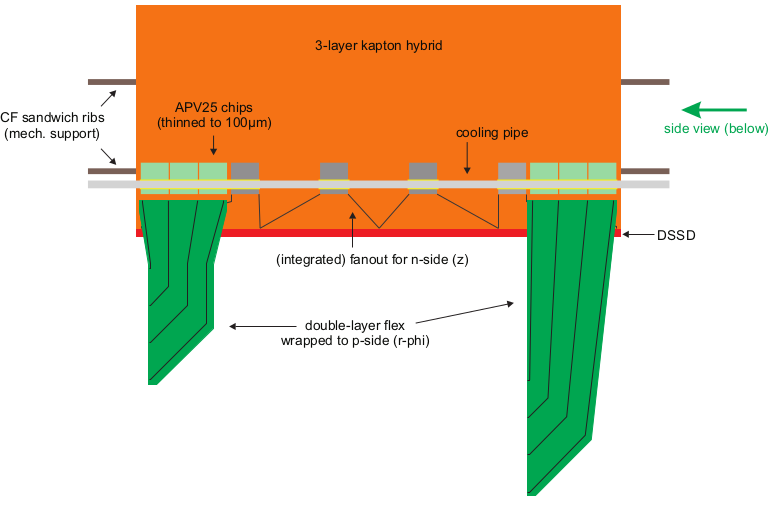
\includegraphics[width=1\linewidth]{ori1}
	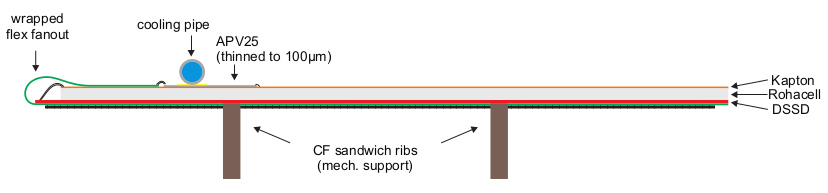
\includegraphics[width=1\linewidth]{ori2}
	\caption{The top and side views of Origami chip-on-sensor design for DSSDs of SVD. Top: the APV25 chips in grep read out the same side sensors channel while chips in green read out the sensors on the opposite side using wrapped-around flex pieces. Bottom: side view of the Origami design shows the location of wrapped flex which connects the strips of the bottom sides which are placed at the left edge~\cite{Abe:2010gxa}.}
	\label{fig:origami}
\end{figure}



\section{Central drift chamber (CDC)}
The central drift chamber (CDC) is the core component of spectrometer in the Belle II that consists of a fairly big drift chamber made of many small drift cells filled with gas. The chamber
gas is comprised of a He–C$_2$H$_6$ 50\%:50\% mixture with an average drift velocity of 3.3 cm $\mu$s$^{-1}$ and a
maximum drift time of about 350 ns for a 17 mm cell size.
The outer radius of CDC has been extended to 1130 mm from 880 mm of Belle, owed to a new thinner particle identification detector which will be introduced in the next section. The whole CDC contains 14336 sense wires in 56 layers, placed in the axial direction and the stereo direction~\cite{b2book}\cite{Abe:2010gxa}. Such a design can utilize the information from axial and stereo wires to construct a full 3 dimensional hits which reflects helix tracks in the CDC volume. Thus, CDC is one of the key components for measuring the helix parameters for tracking, providing precise information on the charged tracks momentum. Also, it provides particle identification information using measurements of energy loss within its gas volume. Low-momentum tracks, which do not reach the particle identification device, can be identified using the CDC alone. Last but not least, it provides efficient and reliable trigger signals for charged particles.

The Belle II CDC is expected to handle higher trigger rates with less dead time. The front-end electronics are located near the backward end-plate and send digital signals to the
electronics hut through optical fibers. Due to the higher radiation and higher beam background in the Belle II, also to create more space for SVD volume, the inner radius of CDC in Belle II is 160 mm. CDC can also create three dimensional trigger information from a dedicated trigger type called $z$-trigger~\cite{Abe:2010gxa} based on the 3D tracking achieved by an FPGA using axial and stereo wires.

The structure of CDC consists of three main components which are a thin carbon-fiber reinforced
plastic (CFRP) inner cylinder, two aluminum endplates, and a CFRP outer cylinder, as shown in Figure \ref{fig:cdc_full}. The outer cylinder is a thickness of 5 mm structure supporting most of the wire tension of 4 tonnes. The inner cylinder is as thin as 0.5 mm to minimize the material and support small cell chamber such as the layers in the inner most region. 

\begin{figure}[htpb]
	\centering
	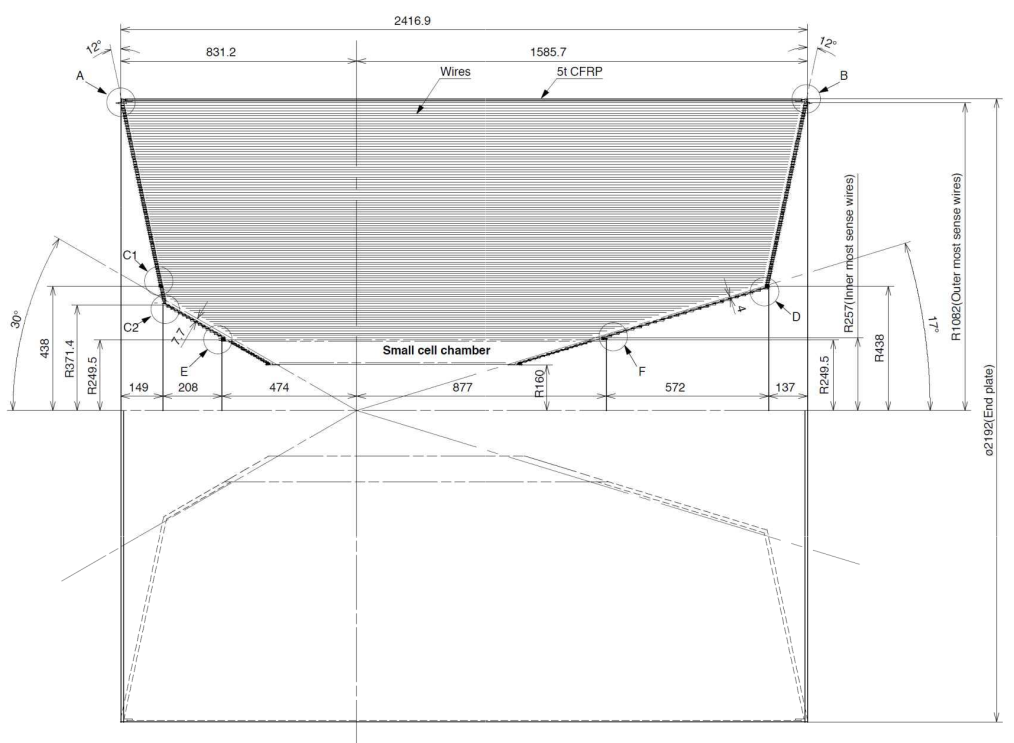
\includegraphics[width=1\linewidth]{cdc_full}
	\caption{CDC structure schematic view \cite{Abe:2010gxa}.}
	\label{fig:cdc_full}
\end{figure}





\section{TOP and ARICH detectors}
The particle identification (PID) system of the Belle II mainly consists of two parts, time-of-propagation counter (TOP) and aerogal based Cherenkov radiation imaging ring (ARICH).

TOP is the specialized detector that can reconstruct Cherenkov radiation time of arrival and generated position by a photon detector placed at the end of a 2.6 cm quartz bar. The TOP is placed at the barrel region of the spectrometer, as shown in Figure \ref{fig:belle2_view}. The conceptional view and the working principle of TOP counter are shown in Figure \ref{fig:top}. In this counter, the time of propagation of the Cherenkov photons that are internally
reflected inside a quartz radiator is measured. The quartz radiator is composed of three components. The first is a long bar for radiating Cherenkov photons. The photons then propagate via total internal reflection towards the bar end, where the MCP-PMTs are mounted. The second is a spherical mirror installed on the forward end of the bar for focusing the photons. The third is a prism that attaches to the backward end of the bar which allows the Cherenkov ring image to expand before the photons are recorded by the PMTs. By this structure, a 3-dimentional information with $x-y$ position and a timing information are obtained by micro-channel plate (MCP) PMTs at the end surfaces of the quartz bar.
The resolution of starting time is achieved about 50 ps~\cite{Abe:2010gxa}. As the key component of the photon detector, the squared shape MCP PMTs, donated as SL-10~\cite{inami2008cross}, have been developed with a $4\times 4$ anode array, a multi-alkali photocathode,
two MCP plates with 10 $\mu$m pore size, and an aluminum layer on the second MCP to protect
against ion feedback. The image of a SL-10 MCP PMT and an anode schematic view are shown in Figure \ref{fig:mcppmt}. 

\begin{figure}[htpb]
	\centering
	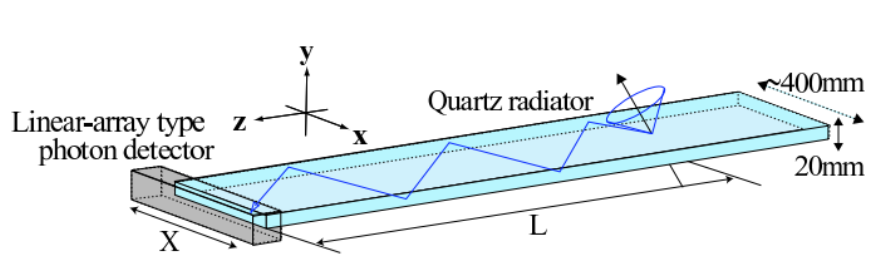
\includegraphics[width=0.7\linewidth]{top_mod}
	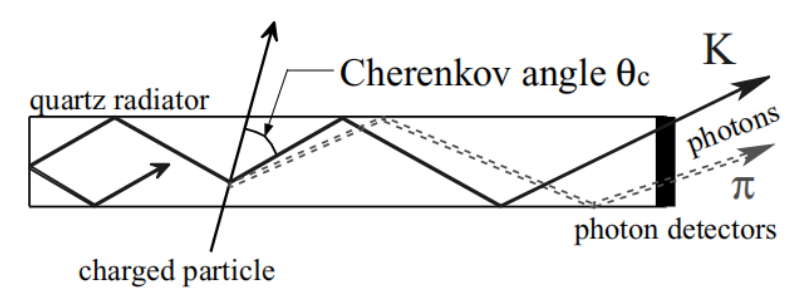
\includegraphics[width=0.7\linewidth]{top_img}
	\caption{Conceptional view of TOP counter (up) and its imaging process of $K^{\pm}$ and $\pi^{\pm}$ (down)~\cite{Abe:2010gxa} for PID purpose.}
	\label{fig:top}
\end{figure}

\begin{figure}[htpb]
	\centering
	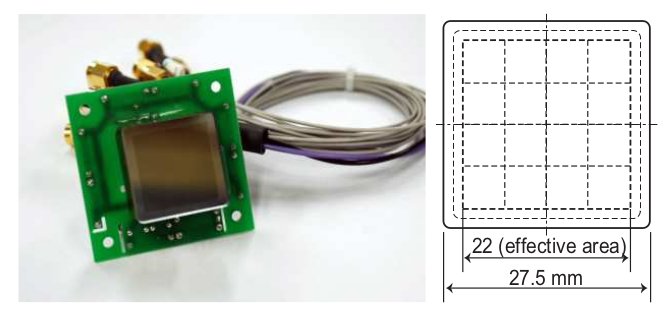
\includegraphics[width=0.8\linewidth]{mcppmt}
	\caption{SL-10 MCP PMT (left) and the schematic view of $4\times 4$ anode (right)~\cite{Abe:2010gxa}}
	\label{fig:mcppmt}
\end{figure}

Aerogel Ring-Imaging Cherenkov
detector (ARICH) is located at the forward endcap in Figure \ref{fig:belle2_view} to separate charged particles in a momentum range from 0.5 GeV/c to 4 GeV/c, which requires a single-photon-sensitive high-granularity sensor to reconstruct the Cherenkov angle with small photon yield.  
Hamamatsu company and the hardware experts from the Belle II collaboration have developed a hybrid avalanche photon detector (HAPD) to meet the requirements. Each sensor is $73 \times 73$ mm$^2$ embedded with 144 channels to accelerate emitted electrons in a 8 kV field. Avalanche photo-diodes (APD) are used for the detection of electrons at the end of electron acceleration, see Figure \ref{fig:arich_img}. The ARICH detector outlook and the ring image of cosmic muon on the HAPD sensors are shown in Figure \ref{fig:HAPD}.

\begin{figure}[htpb]
	\centering
	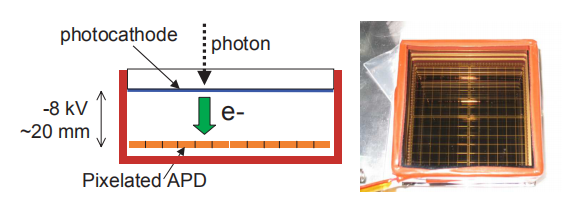
\includegraphics[height=5cm]{HAPD}
	\caption{Photon-electrons acceleration (left) and pixelated APD (right) at the end~\cite{Abe:2010gxa}.}
	\label{fig:arich_img}
\end{figure}



\begin{figure}[htpb]
	\centering
	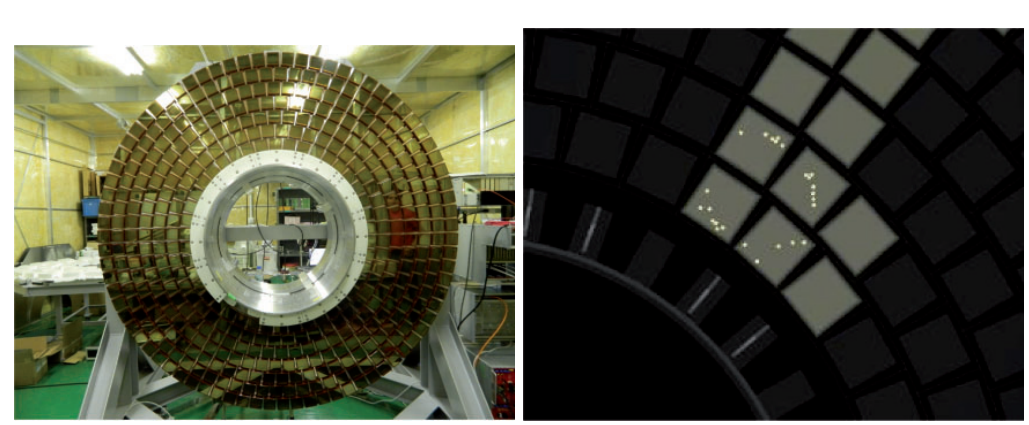
\includegraphics[height=6cm]{ARICH}
	\caption{ARICH detector (left) and the ring image of cosmic muon on the HAPD sensors\cite{b2book}.}
	\label{fig:HAPD}
\end{figure}

\section{Electromagnetic calorimeter (ECL)}
The electromagnetic calorimeter (ECL) in the Belle II is mainly responsible for the detection of $\gamma$ radiation and electrons, providing energy deposition information for trigger, particle reconstruction and PID. ECL consists of three sections as shown in Figure \ref{fig:belle2_view}: a 3 m long barrel section with an inner radius 1.25 m, and two annular endcaps at $z = 1.96$ m (forward) and $z = -1.02$ m (backward) from the IP. The barrel section contains 6624 CsI(TI) crystals of 29 distinct shapes and each crystal is a pyramid shape with about $6\times 6$ in cross section and 30 cm in length. The endcaps section contains 2112 CsI crystals of 69 shapes and the total number of crystals is 8736, with a total
mass of about 43 tons~\cite{Abe:2010gxa}.

As the basic component of ECL, the  thallium doped caesium iodide CsI(TI) crystals are assembled tightly in end-caps and barrel sections. Compared to the previous ECL in Belle, the pre-amplifiers and the structures remain unchanged, while the readout  electronics have been upgraded. The estimated background level in Belle II ECL will cause the much longer decay time in the scintillation of CsI(TI). This will lead to the pile-up effect of readout noise. To compensate this effect, wave-form sampling electronics are embedded with the photon detectors (PMT).
 
\begin{comment}
Especially in the forward direction of the electron beamline, where the level of beam background is much higher, the effect of pile-up noise becomes even worse and the performance of ECL will be of trouble if no special measure taken. Therefore, the pure CsI crystal is considered to be chosen as the material of detector to achieve a fast wave-shaping time and higher radiation tolerance compared to the dosed CsI(TI), which is an back-up option for the future upgrade. ECL is the most important detector for providing trigger information for low multiplicity events, since the main feature of these events is one or two energetic photon(s) emitted from IP region while the charged tracks are missing. 
\end{comment}
  

\section{$K_L^0$ muon detector (KLM)}
The $K_L^0$ and muon detector (KLM) system of the Belle II consists of a sandwich stacked iron plates at outside of the superconducting solenoid and it acts as a return york of the magnet. The iron plates serve as the interaction materials with $>$ 3.9 times the interacting length of material ($\sim 132.1$ g/cm$^{2}$) compared to the ECL, allowing $K_L^0$ particles to shower through. The octagonal barrel covers the polar angle range from 45 degrees to 125 degrees, while the endcaps extend
this coverage from 20 degrees to 155 degrees. There are 15 detector layers and 14 iron plates in the barrel and
14 detector layers and 14 iron plates in each endcap. The side view of KLM is shown in Figure \ref{fig:klm}.
The Belle KLM material uses the glass-electrode resistivity plate chambers (RPC) which is not suitable for the Belle II due to high background level.  Neutrons dose is significantly larger due to the much more electromagnetic radiation reaction on detector materials. The long dead time of RPC under such dose rate will reduce the efficiency of KLM. To mitigate this problem, the RPCs are replaced by the layers of scintillator strips with wavelength-shifting fibers, read out by silicon photomultipliers (called ``SiPMs", Geiger mode operated APDs) as light sensors, which is proven to be able to reliably operate by setting up the discrimination threshold~\cite{b2book}.

\begin{figure}[htbp]
	\centering
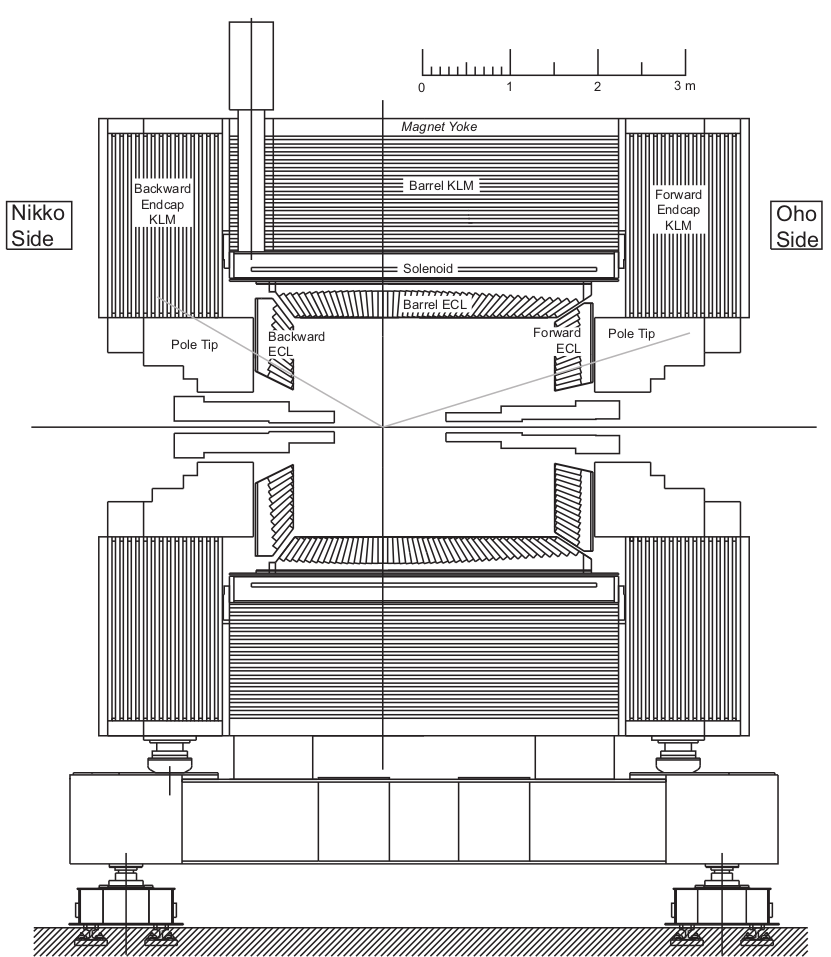
\includegraphics[width=1\linewidth]{klm}
\caption{The side view of KLM in between the ECL and the solenoid, which the grey lines presents the nominal acceptance angle of the Belle II~\cite{Abe:2010gxa}. }
\label{fig:klm}
\end{figure}




\section{Trigger and DAQ system}
The interesting topics in Belle II physics analysis highly depend on the trigger system. The Belle II trigger system is composed of two levels: a hardware-based, low-level trigger called ``L1" trigger, and a software-based high-level trigger (HLT). The L1 trigger has a latency of $\sim 5~ \-\mu\text{s}$ and the maximum trigger output rate is 30 kHz, which is limited by the read-in rate of data acquisition system (DAQ). Considered the high event rate and background level from future Belle II luminosity, a series of upgrades have been implemented for L1 trigger. The key improvements of L1 come from the firmware-based reconstruction algorithm and trigger logic.

The HLT, as the second level of Belle II trigger systema, plays an important role in DAQ. As discussed in the section of PXD, the data size in PXD is huge at high luminosity and the ROI selection must be applied to reduce it. The HLT will first use fast online tracking by CDC and ECL information to further reject the residual beam background not found by L1 trigger. Only the events passing this step are considered for the full event reconstruction. Then the information from all detectors except for PXD are fed into the first event builder for full event reconstruction. The event rate is reduced to about $6$ kHz by HLT which uses the full reconstruction information to find track-associated hits on PXD, introduced as ROI before. The workflow of DAQ with HLT is demonstrated in Figure \ref{fig:daq}. The reduced event rate by applying ROI finding on PXD and other detector read-out systems are combined into the second event builder and eventually written to the offline storage. 

\begin{figure}[htbp]
	\centering
	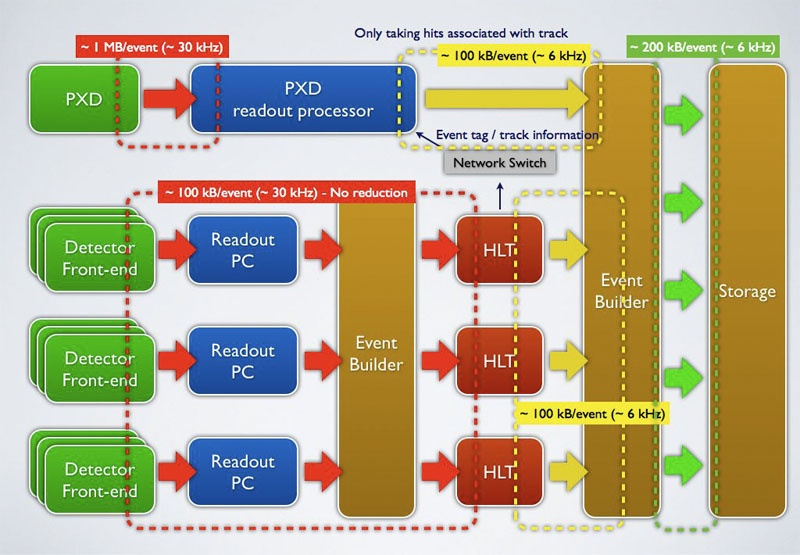
\includegraphics[width=0.8\linewidth]{Belle2DAQ}
	\caption{The Belle II DAQ workflow with HLT between two event builder to reduce the original 30 kHz event rate down to about 6 kHz for offline storage.}
	\label{fig:daq}
\end{figure}


%2021/02/16 ends
Since the primary goal of the Belle II is focusing on $B$ physics studies, it is natural that the trigger system should be able to operate over all of the interesting $B$ physics conditions, with normally 3 or more CDC tracks and large energy deposition in ECL. By studying the efficiency using the simulated events, close to 100\% $B$ decays are recorded by Belle II trigger system. Besides, the Belle II detector is expected to capture many other physics events such as searching for leptonic flavor violation using $\tau$ decays or dark matter particles, of which the performance is highly affected by the beam background level and trigger efficiency. Therefore, the control of beam background becomes essential, which mainly consists of beam-gas scattering, synchrotron radiation, the radioactive Bhabha scattering, the two-photon process, beam-beam effects, and Touschek effect. Their impacts depend on many factors such as beam current, luminosity and vacuum conditions, etc. One of the featured topology of these beam background events is the combination of two charged tracks in CDC and one or two clusters in ECL. The sources of the main beam backgrounds and their event rates in simulation are listed in Table \ref{tab:BG}.

\begin{table}[htbp]
	\centering
	\large
	\caption{Simulated beam background rate~\cite{b2book}}
	\label{tab:BG}
	\begin{tabular}{c c c}
		\toprule
		Type & Source & Rate (MHz)\\
		\hline
		Radiative Bhabha & HER &  1320\\
		Radiative Bhabha & LER &  1294\\
		Radiative Bhabha(wide angle) & HER &  40\\
		Radiative Bhabha (wide angle) & LER &  85\\
		Touschek scattering & HER &  31\\
		Touschek scattering & LER &  83\\
		Beam–gas interactions & HER &  1\\
		Beam–gas interactions & LER &  156\\
		Two-photon QED & - & 206\\
		\bottomrule
	\end{tabular}
\end{table}
\begin{comment}
The improvements on both L1, HLT and the DAQ system are dedicated to serve the operation of the Belle II detector with much higher event rate in future. The further upgrades are also considered such as the replacement of the current DAQ module (COPPER board\cite{Abe:2010gxa} on the read-out PCs) with the latest PCIe-40 platform\cite{mitra2016gbt} to enlarge the bandwidth between detector front-end electronics and the event builder in Figure \ref{fig:daq}.
\end{comment}



\begin{comment}
Based on the reasons discussed above, Belle II trigger has been designed to have 2 separated levels of triggers. Low level trigger, also called as L1 trigger, is hardware-based trigger. and high level trigger (HLT) is the software based trigger.
The L1 trigger rate can go up to 30kHz that is also the up-limit of DAQ read-in rate. The latency of L1 is control to be 5 $\mu$s, improved from Belle trigger.
And yet 30kHz is still to high for writing out the data to tape, so the HLT must be implemented to reduce the trigger rate to about 10kHz and it has to be able to select ROI on the PXD to reduce the data flux limited by bandwidth of read-out cables. To do that, HLT utilize  the full offline reconstruction algorithms to allow the access of full-granularity
event reconstruction using all detectors except for the PXD. 

\end{comment}

%2021.01.27 ends here
\begin{comment}
\section{Detector simulation}
The Belle II simulation makes a use of GEANT4 software. GEANT4 package can accept the event created by module called ``particle gun" which directly injects particles to detector volume. Or it takes in software simulated data, which in general is called ``event generator". Belle II Analysis Framework (BASF2) software (see the next section for the details of BASF2) provides the interface for createing simulated data from event generator to GEANT4. Most of the primary particles are simulated by event generator and sent to GEANT4 for simulation between detectors' components. The out-flying particles that has relatively long life time compared to the primary interaction such as $K_S^0 \to \pi^+ \pi^-$ are simulated in GEANT4 after the event generator does its job. Exchanged bosons and primary electrons(positrons) will not be feed into GEANT4. Then GEANT4 creates secondary particles during the particle interaction and detector material, such as the radiations from charged tracks and also the scattering processes with detector materials. The hits digitization are generated by other BASF2 modules using primary and secondary particles together. Finally, the response from detectors are sent to the persistent data storage (called ``DataStore" as C++ objects, detail in next section.) to be used in the analysis chain of BASF2. 

For each type of the particles and each type of detector material, the interaction is varied in different processes. The co-responding process of physics should be specified by the users or using the provided list from GEANT4 developer group. In Belle II simulation, the
Fritiof quark–gluon string model at high energy and the Bertini intra-nuclear cascade model at low
energy are used by default from GEANT4 list. 

The simulation of the beam background is done by a software called SAD, as external part of BASF2. It simulates the flux of particles from the beamline of the SuperKEKB accelerator. Whenever a particle trajectory deviates from the beamline region and hit the Belle II detector part, its momentum and position vectors will be saved into a configuration file. Then such configuration file will provide the initial information for GEANT4 simulation software to simulate the interaction between the given particle and Belle II detector, which is eventually analyzed as normal particles by BASF2.
The output of BASF2 is standard ROOT format and it presents how a beam induced particle interacts with detector material to create simulated hits as beam backgrounds. 

The mixing of background is then implemented to provide a realistic view of physical events and beam background overlay. Since the format of beam background is simulated hits, thus adding the background events is done by injecting the simulated hits, then move to the digitization of hits to detector responses. In a event time window $\Delta t$, assuming the given type background has a average rate of $R$, the mixing number of background hits in such event is: 

\begin{equation}
\bar{N} = sR\Delta{t}
\end{equation}

$s$ is optional scaling factor which can be used to study the influence of given type background in different level. Because $R$ is averaged value, in the actual mixing, the number of $\bar{N}$ is used as the expected value of Poisson distribution, which presents the number of observed events when many trials of such events is made with certain small possibility per event.  In order to simulate the effect of timing different of background and physical events, the mixing timing window over $\Delta t$ is randomly shift according to the physical events.
With the real experimental data comes in handy, the method of adding background events to physics events is slightly different since using real beam background can provide a more precise result than simulation. By setting a random trigger for beam background, the hits digitization from real beam background will be collected and add to simulated physics events. Although the pile-up noise collected in this method is not very precise because of the threshold set for detectors allowing only part of noise to be added, the non-recorded noise can still contribute to the pile-up noise for physics events, and they are not included in this method. Yet overall it provides a more realistic evaluation of beam background overlay.

\end{comment}

\section{Analysis software framework} 
The data acquired by the Belle II experiment or simulation can be processed by the Belle II Analysis Software Framework, called BASF2. It has a good capability to handle multiple tasks for the Belle II data analysis, from the simulated data production to physics events reconstruction. The BASF2 takes the advantage of good efficiency and reliability of C++ as the programming language, but the use of
Python is also encouraged when it shows clear advantages, such as steering the analysis workflow. 

 %The official BASF2 is developed in different release versions, light-versions and featured-versions. In this thesis, release-05-01-01 version is used. 

\subsection{BASF2 Core Structure}
The core structure of BASF2 contains three major parts: the analysis packages required by the needs of analyzing the Belle II data such as finding tracks and combining particles, the external libraries as the third-party software such as ROOT~\cite{ROOTcern}, and the tools for configuring and installing BASF2 which are mostly Python and shell scripts. Data analysis is supported by providing
a series of modules belonged to BASF2 for appropriate reconstruction based on their specific
needs. To realize this, a modular analysis workflow, where each module can handle the event
data through an unified method such as ROOT I/O based object persistency, is desired. Other
processes, such as data summary table (DST) processing, simulation of each sub-detectors, and data skimming, are done with the packages built for sub-detectors.

The packages are categorized based on the different levels of Belle II detector components, like the packages of base-level system control called ``framework", the package that provides the simulation of each sub-detectors like ``svd",  the package for track reconstruction called ``tracking",  and the package for post-reconstruction data analysis called ``analysis", etc. Users can work either with compiled binary version of BASF2 installed centrally on working servers, or build from the source based on their own need. Furthermore, the distributed computing is also supported by the installations of BASF2 through the managment service provided by DIRAC system~\cite{dirac}. The detail information about the core structure of BASF2 can be found in Ref.~\cite{kuhr2019belle}. 




\begin{comment}
As for the externals, it contains the many packages or libraries that provide functionalities BASF2 needs during the execution or installation. For example, some basic packages, like gcc compiler, cmake, tar, wget, Python and git are included. In particular, due to the dependence of the analysis tools that may be frequently used by Python, around 100 additional Python packages are installed as the externals, such as ``Numpy" and ``matplotlib" packages that provide functions for statistical calculations and plotting. The complexity of building all of these external software could be tough for users so that the compiled versions that cover the common platforms are available from BASF2 official repository. 
Tools are collections of shell or Python scripts for setting up BASF2 and externals environment. It can easily handle the need of setting up an environment of specific BASF2 version and the externals tied to that version. It also provides a function to setting up the environment of developing BASF2, where developers can get one developing copy of BASF2 and write the additional codes as the modification, so the compatibility of BASF2 could be easily maintained by building a release version from the developing branches. In this thesis, two new packages are developed and built with release-05-01-01 version BASF2. This developing version of BASF2 contains all functions that release-05-01-01 has. The details will be discussed later. 
\end{comment}

\subsection{Event processing workflow}
The data from Belle II detector or from the simulation, are organized into a set of runs that are defined by either experimental conditions or simulation conditions. For instance, the simulation data from the condition of a certain detector is packed together, marked with the condition database index used during the simulation.  Such data sample then is divided into different runs based on estimated luminosity from experiment, which can contain the different number of events in each run.  This scheme is used for categorizing experimental data as well, so that users can easily know which experiment conditions are used. Thus, when BASF2 processes a data set, the functions are called for every event based on different configurations that are corresponding to the different experiment conditions. For example, in a data set where events are recorded with the different magnetic fields, BASF2 can automatically change the configurations of the magnetic fields event-by-event to provide a better track measurement. Based on this idea, all BASF2 functions (called ``modules") are developed based on a python module class which contains following embedded functions to be called at event-based level: 


\textbullet \space initialize: called at the start of processing events to prepare this run, including how many events will be processed and declaration of the buffer space and memory required by this module.

\textbullet \space beginRun: called after the initialization is finished and before the event read-in starts, including setting up database conditions used in this run (run-dependent configurations) or event (event-based configurations).

\textbullet \space event: called when each event is read and start to process. This is the actual processing step, such as perform tracking or combining all daughters to find a mother particle. 

\textbullet \space endRun: called at the end of a run, usually to register all processed information to the storage, such as physics variables from all reconstructed particles.

\textbullet \space terminate: called at the end of the processing of all events, release the buffered space and memory.

BASF2 executes a series of modules loaded dynamically to process the data set for analysis purposes, which is shown as Figure \ref{fig:b2flow}. The selection, configuration and executed order of the modules are defined by a file called ``steering file" written in Python. The modules parameters are attributes which can be set during the runtime using the steering file. 
\begin{comment}
For example, the ``Path" object declared in a steering file stores the sequence of modules that will be executed, to which allow other modules such as ``mdstInput" or ``reconstructDecay" to be added.
Users can use ``boolean" type variable set in ``event" function to create a conditional branch of a ``Path" in case that one event needs to be processed with different modules at the same time. For instance, in the decay reconstruction package, if a decay chain is not fulfilled by missing one particle in the ``event" functions, other back-up decay chains can be checked to see if a successful reconstruction is possible.  
\end{comment}


\begin{figure}[htpb]
	\centering
	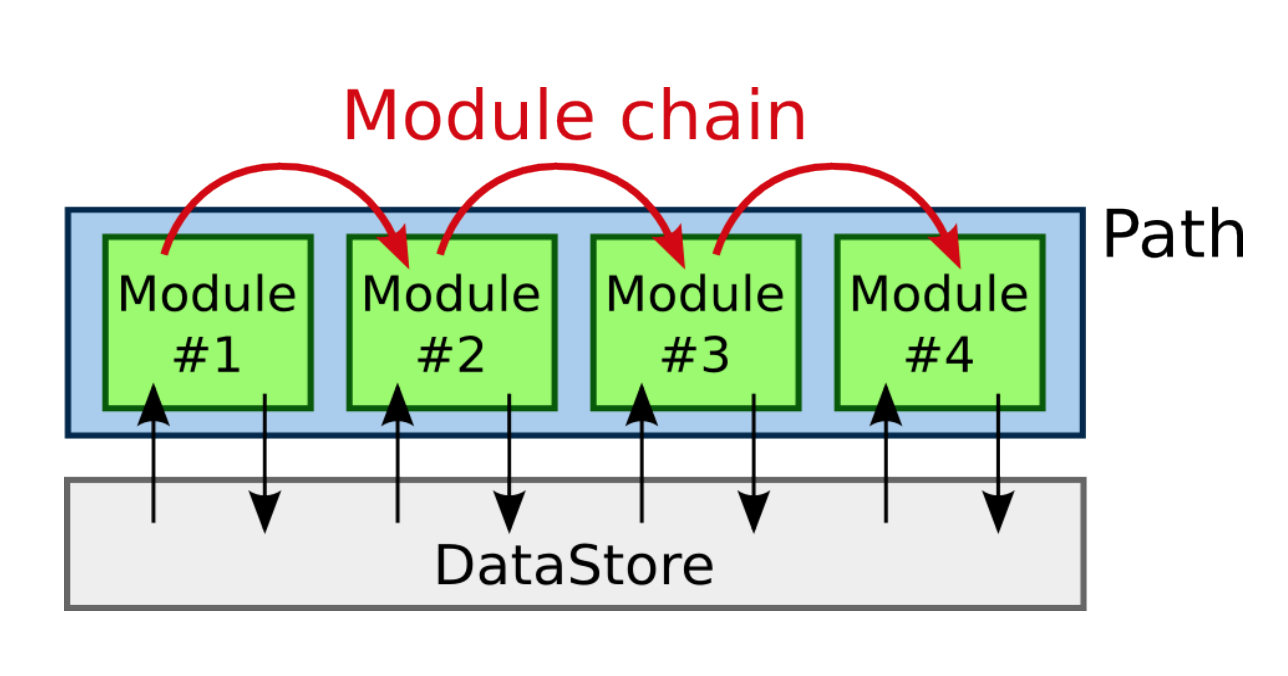
\includegraphics[width=0.8\linewidth]{b2flow}
	\caption{The module-based analysis workflow in BASF2.}
	\label{fig:b2flow}
\end{figure}

The object that interacts with BASF2 I/O is called ``DataStore", as shown in Figure \ref{fig:b2flow}. This implementation doesn't depend on the event data model. The only mandatory component is called ``EventMetaData" which presents the experiment, run  and event number of a event. ``Unpacker" module converts the raw digits into digits-based object in BASF2. In simulation, digitization is done by module called ``digitizer". The digits-based objects are further processed to form hits or clusters depending on detector types. Higher level functions such as tracking and decay reconstructions are implemented based on these basic information by their packages. Eventually, BASF2 writes out the information based on users' needs, like kinematics variables, to ROOT format files, or simply prints out processing statistics to the standard output. 

\begin{comment}
In practice, BASF2 starts running when it checks there is at least one module specifying the number of events to be processed in a ``path"  from the ``steering file", then it reads in the information from DataStore in the input ROOT file, execute all the requested modules in the ``steering file" and return the time and number of events as information printed in standard output.
\end{comment}



\subsection{mDST structure}

The output of BASF2 processing from the online data contains several detector-specific objects, which are restored as mini data summary table (mDST) type ROOT file. For a mDST level analysis, the goal is usually aimed to find particles from physics processes and reconstruct decay information. A output mDST ROOT file contains the reconstructed objects from each sub-detectors, and the following items are required for $B^0 \to K_S^0  K_S^0  K_S^0$ analysis. 


\textbullet \space Track: object presenting any charged particle trajectory. It is linked to multiple track fit results using different nominal mass hypotheses as well as their track fit quality to help select good tracks.  

\textbullet \space TrackFitResult: the fitting result of tracks with different mass hypotheses. It consists of five helix parameters, their covariance matrix and p-value from the fit. It also stores the information of hit pattern on VXD and CDC. 

\textbullet \space V0: object for the relative long-lived neutral particles that fly out of interaction region but mostly decay or interact inside detector region. In Belle II, these are mostly $K_S^0$, $\Lambda$ and photon converted to a electron-positron pair. V0 also stores their relation to the charged daughter tracks and track fit results for further selections.


\textbullet \space PIDLikelihood: it presents for the possiblity of a charged track to be an electron, muon, charged kaon and pion, proton and deuteron provided by particle identification system. 

\begin{comment}
\textbullet \space ECLCluster: reconstructed cluster in ECL detector. It consists of energy deposition and hit positions as well as other hit shape related variables. If a cluster is matched with an extrapolated track, a relation between them will also be created. 

\textbullet \space Reconstructed cluster KLM detector. It consists of momentum and position measurement. If a cluster is matched with an extrapolated track, a relation between them will also be created. 

\textbullet \space KLId: $K_L^0$ candidates with the particle identification as related to KLM and ECL clusters. 

\textbullet \space TRGSummary: L1 trigger information. 

\textbullet \space SoftwareTriggerResult: HLT information mapped by trigger names to trigger results. 
\end{comment}

\textbullet \space  MCParticle: simulated particles and particle-detectors relations are
created if simulated particles are correctly reconstructed as
tracks or clusters.
 

%2020.01.28 ends
\subsection{Conditional Database}

In addition to the physics data, analysis relies on various conditional data that are different calibration of detector, weight files for multi-variate analysis usage like PID and so on. This data is stored in a central database server called central Conditional Database\,(CDB)\,\cite{BASF2}. 
Conditions are made of payloads and each payload has its own``Intervals of Validity" (IoV) which defines in which runs the payload is valid. A collection of the payloads that are produced based on a certain stage of the experiment is packed together and called as a global tag (GT). 
\begin{comment}
A set of payloads and IoVs are called a global tag (GT). Considered the GT that is required by the different analysis purposes may change even though the experiment condition is still same, GT is subjected to be updated once new calibrations of detectors or weight files for analysis tools are available.
\end{comment}


\begin{comment}
On the users' side, except for just using central database, a local database back-end that takes GT information such as calibration data while uses a local database, such as a customized PID weight file,  is also possible.  It automatically download the needed database files that are required for a BASF2 execution and stores them in a local folder. This means even if the local machine is offline or the CDB is not accessible, one can still run BASF2 as long as the local folder is there. 
\begin{figure}[htbp]
\centering
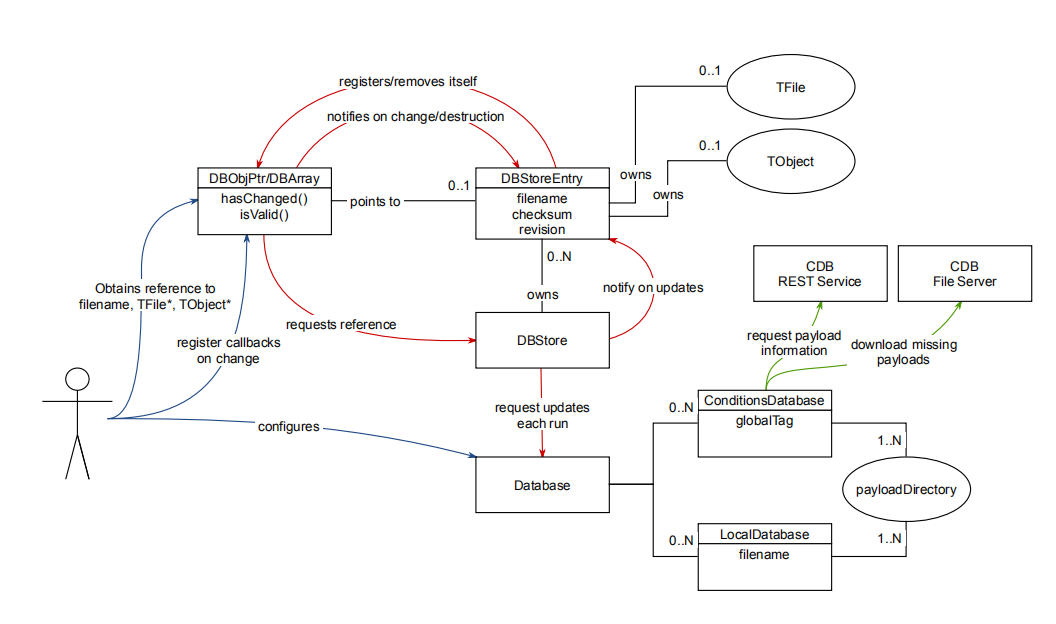
\includegraphics[height=9cm]{CDB}
\caption{ Relations of all entities in CDB\cite{BASF2}, showing the management logic from users' end to each CDB files and services. }
\label{fig:CDB}
\end{figure}
\end{comment}
 



\begin{comment}
The management of CBD with the extension of local database gives a good convenience for users to perform their own analysis and share the results with collaborators.
Users' access to conditions objects in the CDB is
provided by two interface classes, one for single objects
called ``DBObjPtr" and one for arrays of objects called
``DBArray". To facilitate easy creation of new conditions data – for example, during calibration – we provide two payload creation classes, ``DBImportObj" and ``DBImportArray". They
have an interface very similar to DBObjPtr and DBArray\cite{BASF2}.
\end{comment}

Users can create a GT, add objects of payloads to it and commit the GT to the configured database with a user-supplied IoV. This includes the support for run dependency as well. The capability to use a local file-based
database allows for easy preparation and validation of new payloads before they are uploaded to the CDB. Only the creator of the payload objects has the right to add, recall, replace and remove the GT from CDB, which guarantees the stability.

\begin{comment}
The scheme of this entities and how users interact with CDB object is demonstrated in Figure \ref{fig:CDB}. For example, user can perform their analysis and first locally generate weight files or calibration data based on different run conditions and reconstruction criteria, which are stated by their names of the IoVs. Once the results are good to share, they can create a GT in CDB of which they have the full ownership, add all database files into the GT and open it to Belle II collaboration. Anyone who would like to re-calibrate data or use their weight files for PID and so on, can simply use the built-in function ``basf2.useCentralDB()" in the BASF2 steering file to directly access the corresponding data. However, only the creator of the CDB objects has the right to add, recall, replace and remove the GT, which guarantees the stability of the CDB and responsibilities for each user.

\end{comment}

\begin{comment}
\subsection{Summary}
BASF2 has been developed for an emphasis on providing reliable and high quality performance for Belle II analysis. It satisfies the most of demanding requirements of data taking, simulation, reconstruction, and offline analysis. 
\end{comment}

\section{Belle II simulation}

This section briefly describes simulation (MC) used in the studies presented in this thesis. As this analysis is based on neutral $B$ meson, which is from the $\Upsilon$(4S) events, the  simulation is based on the electron -positron collisions at center-of-mass (CMS) energy $\sqrt{s} = 10.58 $ GeV.

In the previous section, it is shown that external packages and functionalities have been integrated with BASF2, including the core components of Belle II simulation in $B$ decay: \textit{evtgen} as event generator~\cite{evtgen} and \textit{GEANT4} as the simulator of detectors~\cite{agostinelli2003geant4}. For the simulation and the reconstruction used in this analysis, the latest release of BASF2 (release-05-01-01) was used. Based on the CDB management, BASF2 can utilize the same constants such as the magnetic field distribution for the consistence between simulation and reconstruction.

 All simulations start with at least one event generator that configures the physics processes. The \textit{evtgen} requires a decay file that describes the decay chain from a certain mother particle, branching fraction for all processes and decay-related information such as flavor mixing or $\it{CP}$ violation information. MC sample is centrally produced using Belle II grid computing service by DIRAC system and skimmed, of which the output is for physics analysis to create ROOT files. Each round of MC sample is packed and marked by their production index, such as \textit{MC13}, which is the latest MC sample with improvements in PID. In the following content of this thesis, all MC samples are produced in \textit{MC13} if not specifically stated. 
 
 For the analysis in this thesis, there are two MC samples included, where one is called \textit{signal MC} and the other is called \textit{generic MC}. \textit{Signal MC}, as its name suggests, is the MC sample that describes the whole decay chain of $B^0 \to K_S^0  K_S^0  K_S^0$. The mother particle of the decay chain is $\Upsilon$(4S), then it decays into a pair of $B^0-\bar{B}^0$ at branching fraction of 100\%, with the model \textit{EvtVSSMix}~\cite{evtgen} describing the decay model. Then, one of the $B^0$ meson is set to decay into three $K_S^0$ based on phase-space model ($PHSP$) at 100\% branching fraction. The default configuration of evtgen can not handle multi-bodies charmless $B$ decay with TDCPV. A modified decay model profile is under-development and not fully validated yet. Thus, MC sample of $B^0 \to K_S^0  K_S^0  K_S^0$ yields zero $\it{CP}$ violation by default. As for the other $B$ meson, it decays into all possible final states that are described by the Belle II generic decay file. 
 
 As for \textit{generic MC}, all hadronic processes in a  $\sqrt{s} = 10.58 $ GeV collision are simulated. The total production cross section receives contributions from not only $\Upsilon$(4S) ($b$-flavor decay dominated), but also $u, d, s, c$. 
 Their relative branching fractions are taken from cross sections at  $\sqrt{s} = 10.58 $ GeV as shown in Table \ref{tab:generic_br}. \textit{Generic MC} sample contains 6 types of MC samples due to this production arrangement, where $\Upsilon$(4S) produces \textit{mixed} (neutral) and \textit{charged} $B$ meson pairs and the rest are other flavor mesons possibly with one extra photon emission named as $u\bar{u}(\gamma)$, $d\bar{d}(\gamma)$, $s\bar{s}(\gamma)$, and $c\bar{c}(\gamma)$, respectively. In this thesis, the latter 4 types of MC samples are combined and called $q\bar{q}$ for simplicity. In the mixed MC sample, the branching fraction of $B^0 \to K_S^0  K_S^0  K_S^0$ is set at $6 \times 10^{-6}$ and the branching fraction of $K_S^0 \to \pi^{+}\pi^{-}$ is set at 0.692. Both values are taken from Particle Data Group (PDG)~\cite{pdg}. As the same as \textit{signal MC}, $\it{CP}$ violation is set to zero for signal events in \textit{generic MC} since they use the same model at generator level.
 
 \begin{table}
 	\caption{Production cross section for different hadronic flavors from collision at  $\sqrt{s} = 10.58 $ GeV used in Belle II \textit{generic MC}~\cite{b2book}.}
 	\label{tab:generic_br}
 	\centering
 	\begin{tabular}{c|c|c|c|c|c}
 		\hline 
 	Processes & $\Upsilon$(4S) & $u\bar{u}(\gamma)$ & $d\bar{d}(\gamma)$ & $s\bar{s}(\gamma)$ & $c\bar{c}(\gamma)$ \\
 		\hline 
 	Cross section [nb] & $1.110\pm0.008$ & 1.61 & 0.40 & 0.38 & 1.30 \\
 	\hline
 	\end{tabular}
 \end{table}
 
In addition to the simulation of physics processes,  simulated data is produced with at least two beam background conditions, called \textit{BG0} without beam background and \textit{BG1} with one overlay of beam background. The components of them have been discussed briefly in section 2.7. The mixing of simulated beam background to simulated physics events is done by adding simulated hits on each sub-detector output. Possible pile-up of hits is therefore inherently included. The average number of background events of a given type to be added to a single simulated event is determined from the rate $R_{BG}$ of beam background sample and the time window $\Delta t$ in which the background is mixed shown in Equation \ref{bkgn}:

\begin{equation}\label{bkgn}
	\bar{N} = sR_{BG}\Delta t
\end{equation}
where $s$ is an optional scaling factor. The injected background events are based on a Poisson distribution with mean $\bar{N}$. Within the timing window, the background events are shifted randomly to simulate contributions from different bunches. To use real experiment background events (data-based beam background), the random triggered events are measured and added to
simulated $BG0$ MC sample for a more precised background configuration. This method can give a more realistic description of actual beam background but with a possibility to introduce bias due to the pile-up effect of multiple background events in a short timing window. In the early stage of the Belle II, the level of background is not high and the background pile-up effect is small.

In total, there are 2 million events generated in \textit{signal MC}. Half of the \textit{signal MC} (1 million) is produced without beam background for cross-checking the reconstruction performance. For \textit{generic MC}, 1 ab$^{-1}$ sample including mixed, charged and $q\bar{q}$ events are produced with beam background at  $\sqrt{s} = 10.58 $ GeV. The MC sample used in this analysis is summarized in Table \ref{tab:mc_all}

\begin{table}
	\large
	\caption{MC samples with and without beam background used in $B^0 \to K_S^0  K_S^0  K_S^0$ analysis.}
	\label{tab:mc_all}
	\centering
	\begin{tabular}{c|c|c}
		\hline 
		Events number & BG0 & BG1 \\
		\hline
		\textit{\textit{signal MC}} & $10^6$ & $10^6$ \\
		\hline
		\textit{\textit{generic MC}} & None & 1 ab$^{-1}$\\
		\hline
	\end{tabular}
\end{table}


\section{Belle II data taking}
The Belle II beam test operation started in 2016 which was focused on the commissioning and test of the SuperKEKB accelerator. Later in 2018, the commissioning of the Belle II detector was accomplished, with partial installation of PXD and full installation of SVD. From 2019 April, the physics run operation has officially started. The rest of the PXD is scheduled to be installed in 2023. By the end of 2020, Belle II has been operating for 4 total run seasons. The integrated luminosity collected during this period of time is about 84.73 fb$^{-1}$, shown in Figure \ref{fig:b2lumi}. The indices of physics runs are labeled which are experiment 7,8,10 for 2019 data taking and experiment 12 and 14 for 2020 data taking, as shown in Figure \ref{fig:b2lumi}. The data processing is regularly performed along with the data taking. For the analysis reported in this thesis, the experimental data collection from experiment 7, 8, 10 and 12 is used. Correspondingly, the integrated luminosity for offline reconstruction used in this thesis is about 62.8 fb$^{-1}$~\cite{b2onlinelumi}. The experiment 14 is not used due to the unfinished processing of the latest experiment data by the time this thesis is composed. 

\begin{figure}
	\centering
	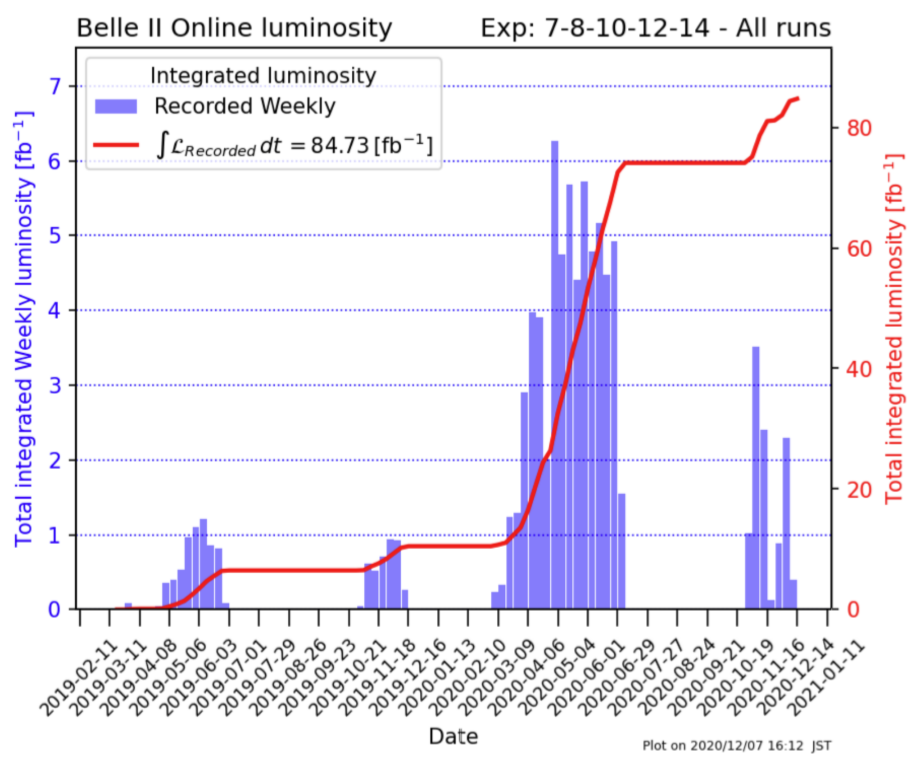
\includegraphics[width=0.6\linewidth]{b2lumi}
	\caption{Belle II online luminosity from 2019 April to the end of 2020. The experiment 7 and 8 were conducted during 2019 March to June. The experiment 10 was conducted during 2019 October to 2019 November. The experiment 12 was conducted during 2020 February to June. The experiment 14 was conducted during 2020 September to November.}
	\label{fig:b2lumi} 
\end{figure}
% 2021.02.01 ends